% -*- coding: utf-8 -*-
\documentclass[a4paper,12pt]{article}
\usepackage[T1]{fontenc}
\usepackage[utf8]{inputenc}
\usepackage[russian]{babel}
\usepackage{amsmath,amsfonts,amssymb}
\usepackage{graphicx}
\usepackage{booktabs}
\usepackage{caption}
\usepackage{float}
\usepackage{geometry}
\geometry{margin=2.5cm}

% Все изображения хранятся в папке Graphics
\graphicspath{{Graphics/}}

\author{~}
\date{}
\title{Случайные графы. Отчет по проекту.}
\begin{document}
\maketitle

%--------------------------------------------------
\section*{Часть 1: Зависимость графовых метрик от параметров распределений}

\begin{figure}[H]
    \centering
    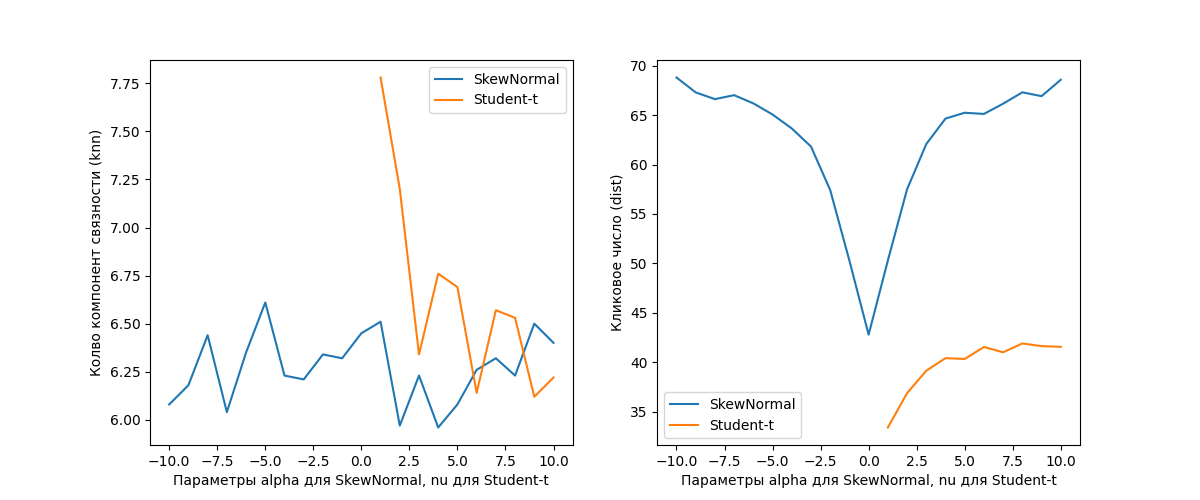
\includegraphics[width=0.95\textwidth]{part1_results_Askar.png}
    \caption{Серия Аскара: SkewNormal vs Student-$t$ при фиксированных параметрах графа ($n=100$, $k=5$ / $d=1$).}
    \label{fig:part1-askar}
\end{figure}

\subsection*{Выводы Аскара }
\begin{itemize}
    \item В kNN-графе параметр $\alpha$ почти не влияет на число компонент связности.
    \item Чем больше $\nu$ у Student-$t$, тем меньше компонент.
    \item В dist-графе при $\alpha\to0$ кликовое число падает, при $|\alpha|$ большим — растёт.
    \item Чем больше $\nu$, тем выше кликовое число.
\end{itemize}

\begin{figure}[H]
    \centering
    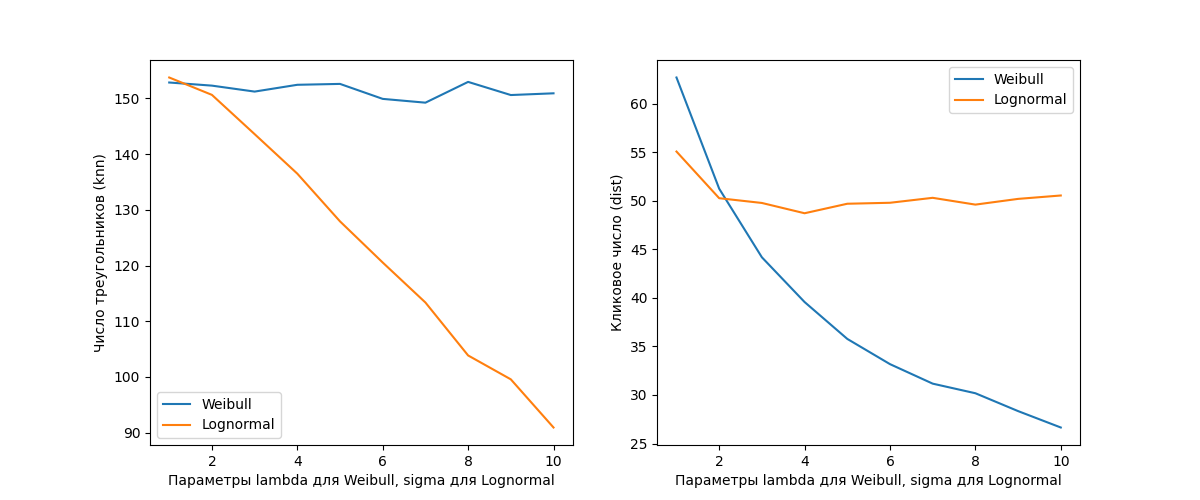
\includegraphics[width=0.95\textwidth]{part1_results_Yaroslav.png}
    \caption{Серия Ярослава: Weibull vs Lognormal.}
    \label{fig:part1-yaroslav}
\end{figure}

\subsection*{Выводы Ярослава }
\begin{itemize}
    \item В kNN-графе параметр $\lambda$ практически не влияет на число треугольников.
    \item Параметр $\sigma$ логнормального распределения обратно пропорционален числу треугольников.
    \item В dist-графе $\lambda$ обратно пропорционален кликовому числу.
    \item Параметр $\sigma$ почти не влияет на кликовое число.
\end{itemize}

%--------------------------------------------------
\section*{Часть 2: Зависимость метрик от $n$, $k$ и $d$}

\begin{figure}[H]
    \centering
    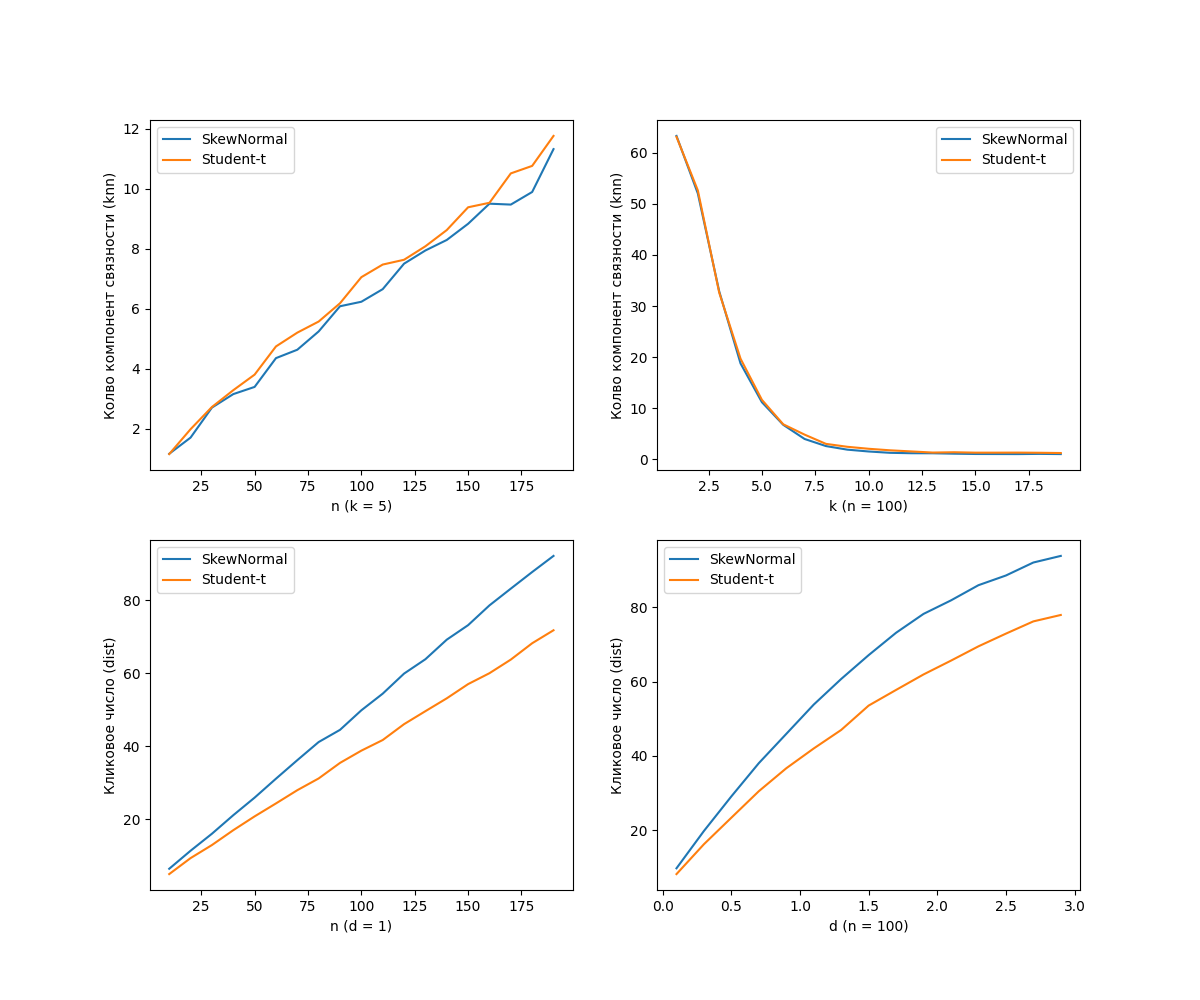
\includegraphics[width=0.95\textwidth]{part2_results_Askar.png}
    \caption{Серия Аскара: изменение $n$, $k$ и $d$.}
    \label{fig:part2-askar}
\end{figure}

\subsection*{Выводы Аскара }
Для dist-графа различия в числовых характеристиках при изменении параметров графа более ощутимы, чем для kNN-графа.

\begin{figure}[H]
    \centering
    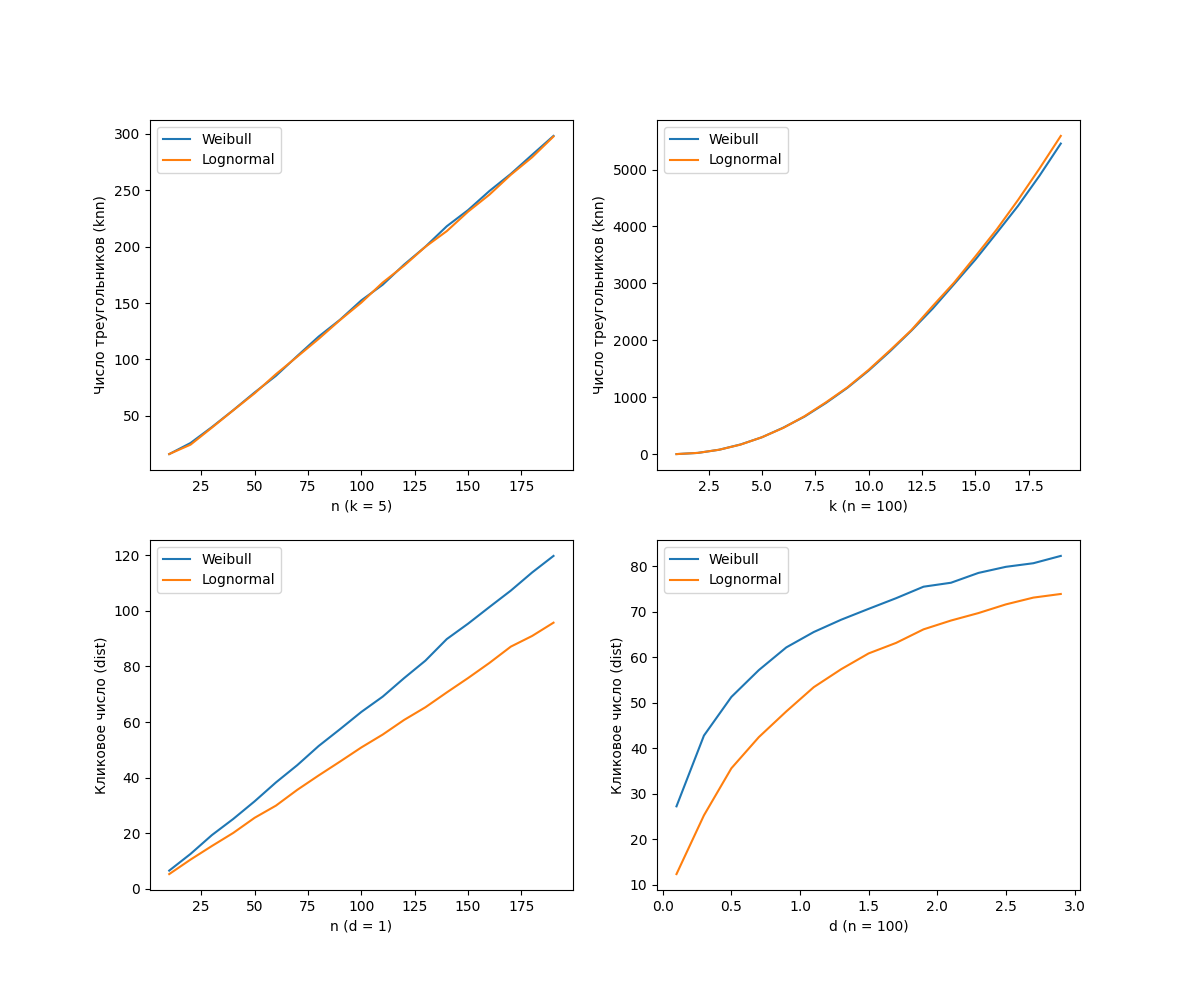
\includegraphics[width=0.95\textwidth]{part2_results_Yaroslav.png}
    \caption{Серия Ярослава: изменение $n$, $k$ и $d$.}
    \label{fig:part2-yaroslav}
\end{figure}

\subsection*{Выводы Ярослава }
KNN почти не реагирует на изменения параметров, тогда как dist-граф демонстрирует усиленные различия; кликовое число Weibull смещено вверх.

%--------------------------------------------------
\section*{Часть 3: Проверка статистических гипотез и оценка мощности}

\begin{figure}[H]
    \centering
    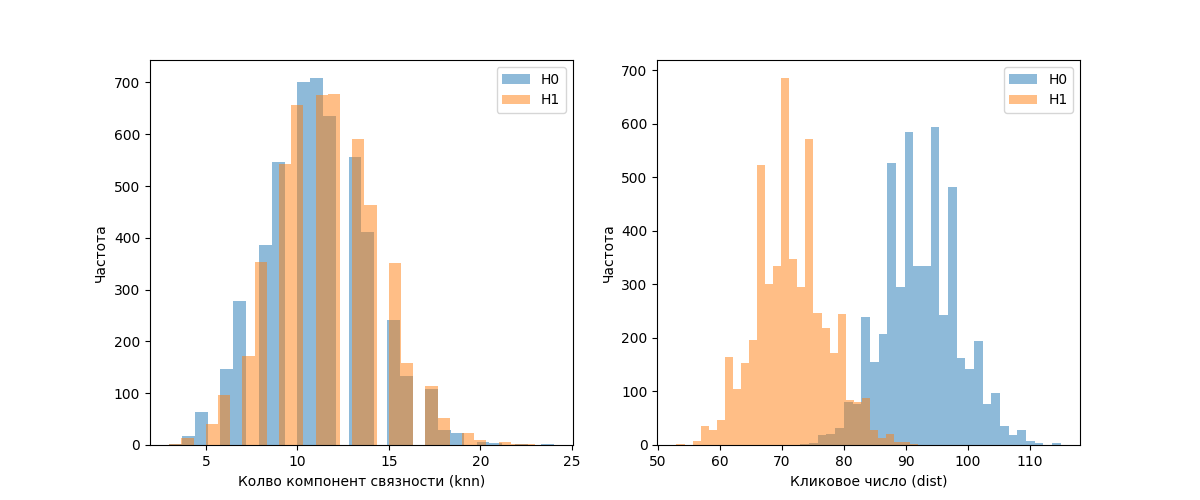
\includegraphics[width=0.95\textwidth]{part3_results_0_Askar.png}
    \caption{Askar: распределения метрик под $H_0$ и $H_1$ (первый набор).}
    \label{fig:part3-0-askar}
\end{figure}

\begin{figure}[H]
    \centering
    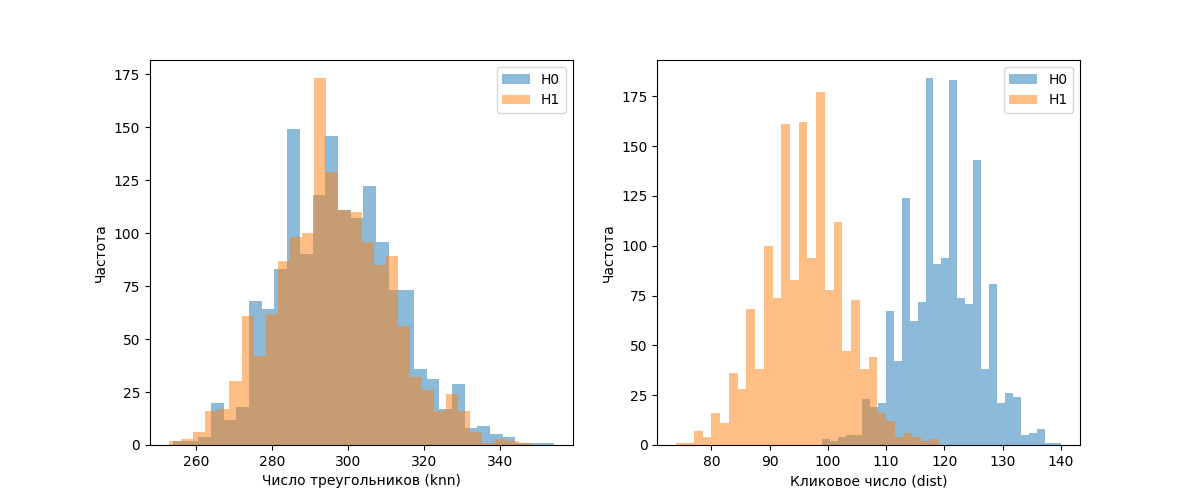
\includegraphics[width=0.95\textwidth]{part3_results_0_Yaroslav.png}
    \caption{Yaroslav: распределения метрик под $H_0$ и $H_1$ (первый набор).}
    \label{fig:part3-0-yaroslav}
\end{figure}

\begin{figure}[H]
    \centering
    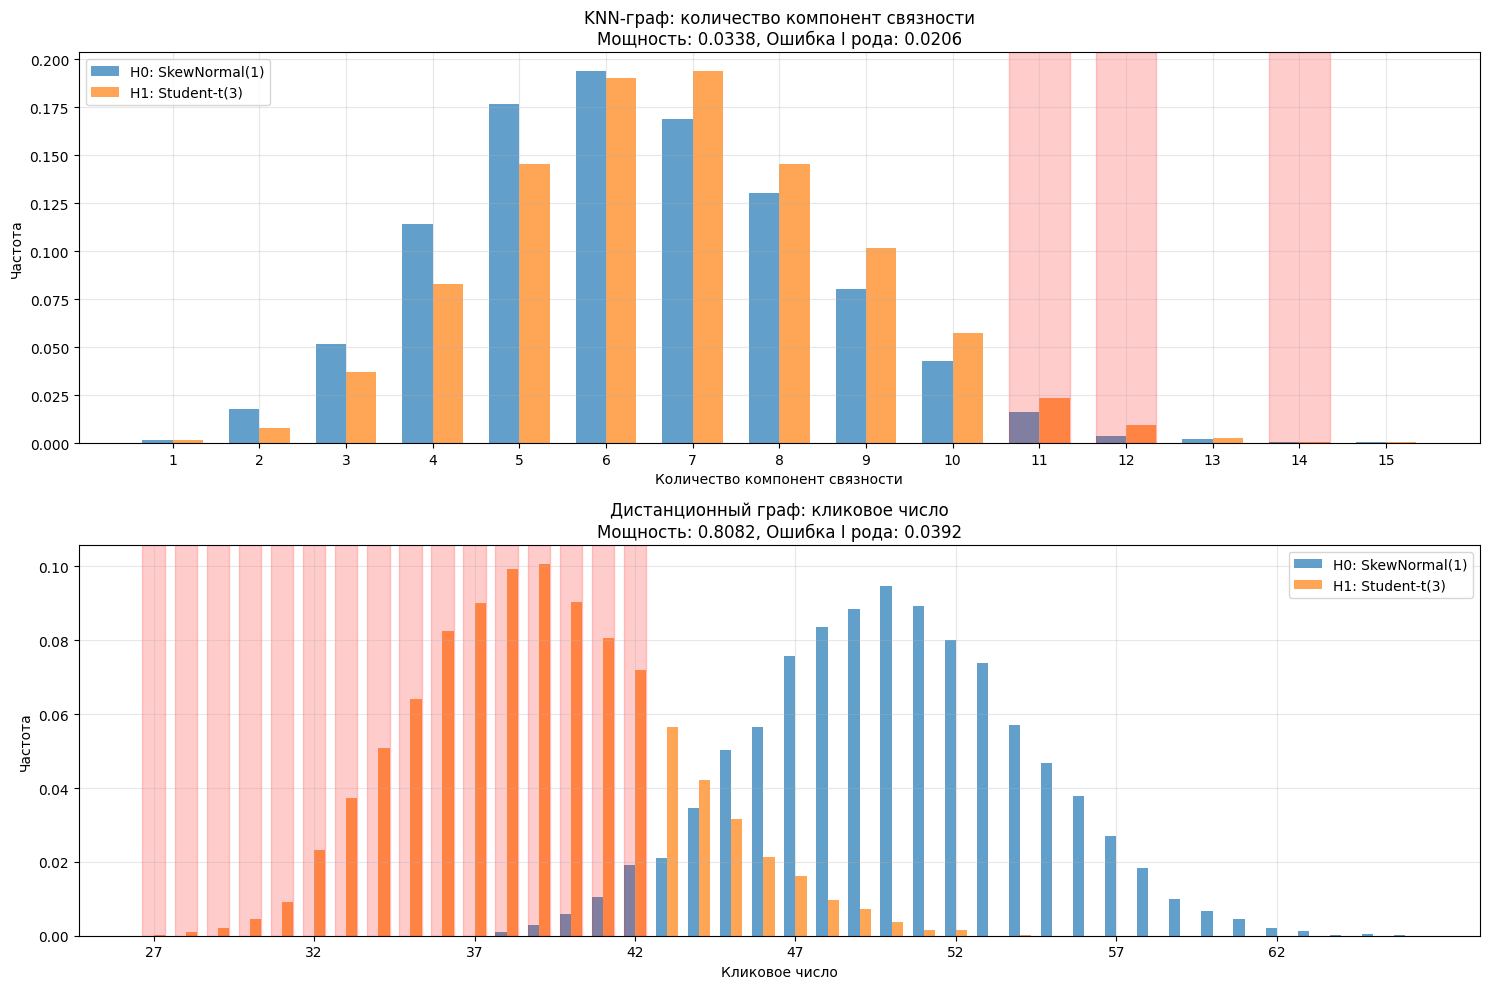
\includegraphics[width=0.95\textwidth]{part3_results_1_Askar.png}
    \caption{Askar: гистограммы с критической областью (второй набор).}
    \label{fig:part3-1-askar}
\end{figure}

\begin{figure}[H]
    \centering
    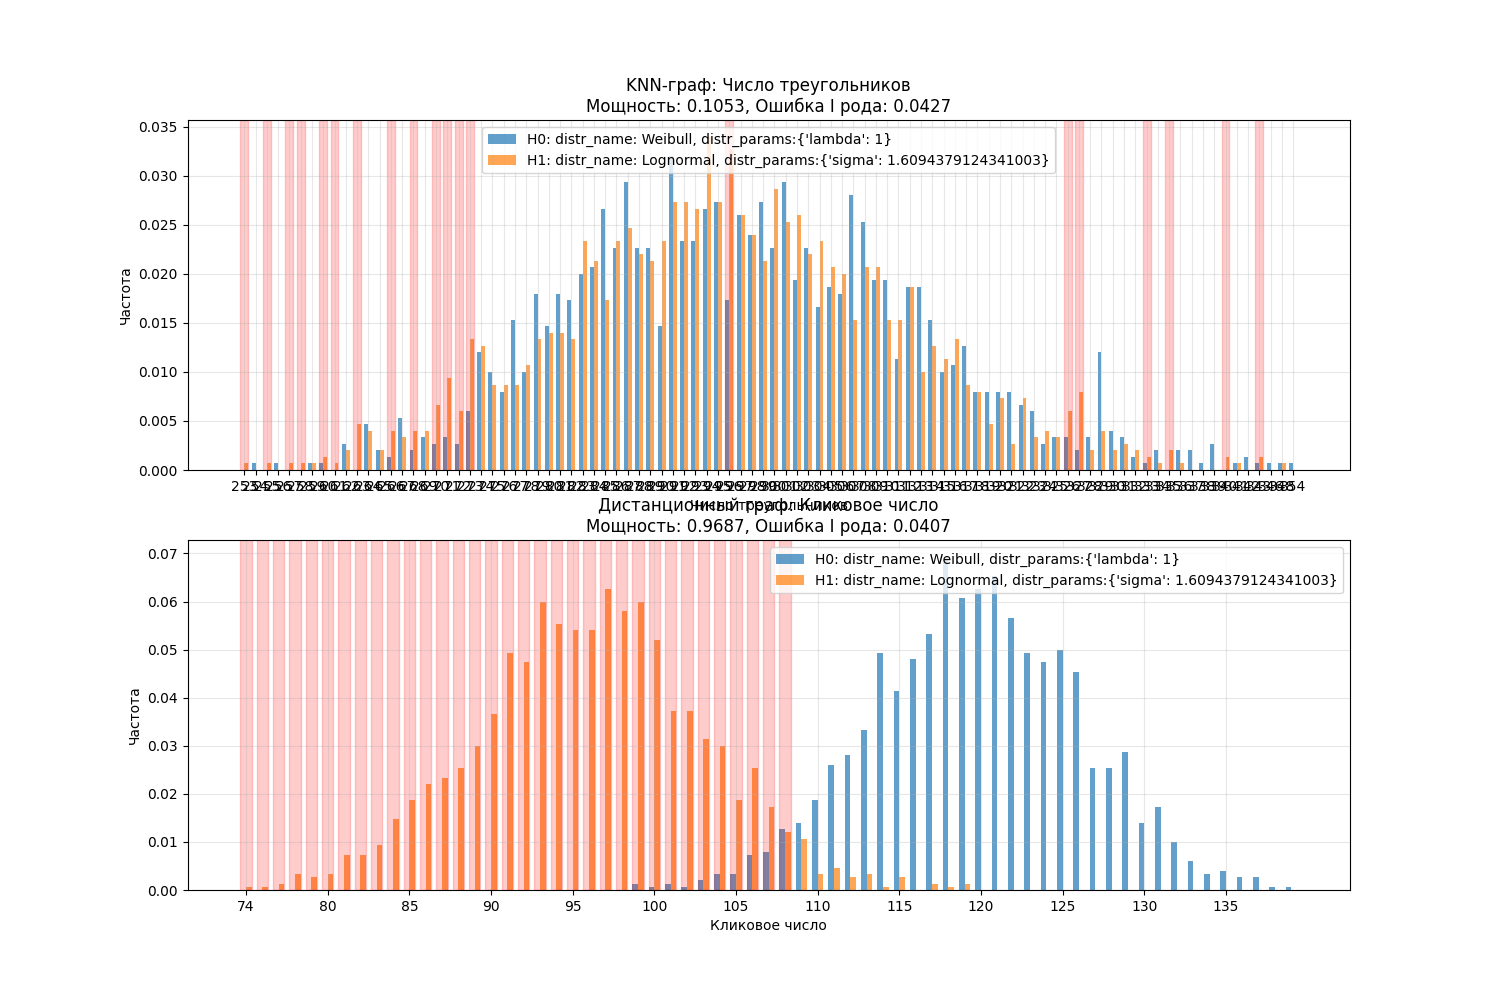
\includegraphics[width=0.95\textwidth]{part3_results_1_Yaroslav.png}
    \caption{Yaroslav: гистограммы с критической областью (второй набор).}
    \label{fig:part3-1-yaroslav}
\end{figure}

\subsection*{Выводы }
\begin{itemize}
    \item Для kNN-графа числовые характеристики (компоненты, треугольники) плохо разделяют гипотезы: распределения $H_0$ и $H_1$ сильно перекрываются.
    \item Для dist-графа характеристика «кликовое число» значительно лучше разделяет гипотезы: наблюдается практически полное разделение распределений.
\end{itemize}

\begin{table}[H]
    \centering
    \caption{Эмпирическая мощность тестов }
    \label{tab:power}
    \begin{tabular}{@{}llll@{}}
        \toprule
        Сценарий & Метрика & Мощность & Ошибка I рода \\
        \midrule
        Askar & Компоненты (kNN) & $0.013$ & $0.007$ \\
        & Клика (dist) & $0.968$ & $0.046$ \\
        Yaroslav & Треугольники (kNN) & $0.105$ & $0.043$ \\
        & Клика (dist) & $0.969$ & $0.041$ \\
        \bottomrule
    \end{tabular}
\end{table}

%--------------------------------------------------

\end{document}
